\documentclass[oneside]{article}
% Título y autor(es):
\title{Resumen de Álgebra II (61.08)}
\author{Menéndez Martín}

\usepackage[spanish]{babel}
\usepackage{amsmath,bm,times}
\usepackage[a4paper,headheight=16pt,scale={0.7,0.8},hoffset=0.5cm]{geometry}
\usepackage{pdfpages}
\usepackage[utf8]{inputenc}
\usepackage{lastpage}
\usepackage{float}
\usepackage{array}
\usepackage{listings}
\usepackage{anysize}
\usepackage{pdfpages}
\numberwithin{equation}{section}
\numberwithin{figure}{section}
\numberwithin{table}{section}
\usepackage{fancyhdr}
\usepackage[hang,bf]{caption}
\usepackage{graphicx}
\usepackage{svg}
\usepackage{pgf,tikz}
\usepackage{tikz-timing}
\usepackage{setspace}
\usepackage{verbatim}
\usepackage{booktabs}

\includepdfset{pagecommand=\thispagestyle{plain}}
\usetikzlibrary{shapes,arrows,positioning,shadows,trees,automata}

\pdfcompresslevel=9
\newcommand{\imgdir}{includes}
\graphicspath{{\imgdir/}}

\everymath{\displaystyle}
\newcommand{\vect}[1]{\overline{\textbf{#1}}}
\newcommand{\bayes}{\mathop{\lessgtr}}

\newcommand{\fil}[1]{\text{Fil}(#1)}
\newcommand{\col}[1]{\text{Col}(#1)}
\newcommand{\nul}[1]{\text{Nul}(#1)}
\newcommand{\rg}[1]{\text{rango}(#1)}
\newcommand{\dime}[1]{\text{Dim}(#1)}
\newcommand{\dete}[1]{\vert #1 \vert}
\newcommand{\tr}[1]{\text{tr}(#1)}
\newcommand{\gen}[1]{\text{gen}\left\{#1\right\}}
\newcommand{\produ}[1]{(#1)}

\tikzstyle{definicion} = [draw=red, fill=gray!20, very thick,rectangle, rounded corners, inner sep=10pt, inner ysep=20pt]
\tikzstyle{fancytitle} =[fill=red, text=white]
					
\tikzstyle{corolario} = [draw=red, fill=green!20, very thick,rectangle, rounded corners, inner sep=10pt, inner ysep=20pt]
\tikzstyle{fancytitle} =[fill=red, text=white]
					
\tikzstyle{teorema} = [draw=red, fill=blue!20, very thick,rectangle, rounded corners, inner sep=10pt, inner ysep=20pt]
\tikzstyle{fancytitle} =[fill=red, text=white]										

%------------------------- Inicio del documento ---------------------------

\begin{document}
% Hago que en la cabecera de página se muestre a la derecha la sección, y en el pie, en número de página a la derecha:
\pagestyle{fancy}
\renewcommand{\sectionmark}[1]{\markboth{}{\thesection\ \ #1}}
\lhead{}
\chead{}
\rhead{\rightmark}
\lfoot{Álgebra II (61.08)}
\cfoot{}
\rfoot{P\'agina \thepage\ de \pageref{LastPage}}
% Carátula:
\begin{titlepage}

\thispagestyle{empty}

\begin{center}

\includegraphics[scale=0.3]{fiuba}\\
\large{\textsc{Universidad de Buenos Aires}}\\
\large{\textsc{Facultad De Ingeniería}}\\
\small{A\~no 2015 - 1\textsuperscript{er} Cuatrimestre}
\end{center}

\begin{center}
\Large{\underline{\textsc{Álgebra II A (61.08)}}}

\vspace*{2cm}

\textbf{\begin{LARGE}
Resumen de Álgebra II\\
\end{LARGE}}
\end{center}

\vspace*{3cm}

\begin{tabbing}
\hspace{2cm}\=\+
\\
	INTEGRANTE:\hspace{-1cm}\=\+\hspace{1cm}\=\hspace{6cm}\=\\
		Maria Inés Parnisari	\>\>- \ 92235\\
		$\langle$maineparnisari@gmail.com$\rangle$\\
		\\
		Menéndez, Martín Nicolás	\>\>- \ 92830\\
		$\langle$menendez91@live.com.ar$\rangle$\\
		\\
\end{tabbing}
\end{titlepage}
% Hago que las páginas se comiencen a contar a partir de aquí:
\setcounter{page}{1}
% Pongo el índice en una página aparte:
\tableofcontents
%\listoffigures
%\listoftables
\newpage
% Inicio del TP:
\marginsize{1cm}{1cm}{1cm}{1cm}
%\setcounter{chapter}{1}

	\section{Matrices}
	
		\subsection{Propiedades generales}
		
				\begin{tikzpicture}
					\node [corolario] (box){%
					    \begin{minipage}{0.80\textwidth}
					   		Dadas las matrices $A,B,C$ se tiene que:\\
					   		
					   		\begin{minipage}{0.4\textwidth}
					   			\begin{itemize}
						   			\item $A+B=B+A$
					   				\item $A+(B+C)=(A+B)+C$
					   				\item $\alpha(A+B)=\alpha A+\alpha B$
					   				\item $(\alpha+\beta)A=\alpha A+\beta A$
					   				\item $\alpha\left(\beta A\right)=(\alpha\beta)A$
					   				\item $A+0_n=A$	   				
					   			\end{itemize} 				
					   		\end{minipage}
					   		\begin{minipage}{0.4\textwidth}	
					   			\begin{itemize}
					   				\item $A+(-A)=0_n$
						   			\item $A(B+C)=AB+AC$
									\item $(A+B)C=AC+BC$
					   				\item $A(BC)=(AB)C$
					   				\item $\alpha(AB)=(\alpha A)B=A(\alpha B)$
					   				\item $A 0_n=0_n$
					   			\end{itemize} 	
					   		\end{minipage}
					    \end{minipage}
					};
				\node[fancytitle, right=10pt] at (box.north west) {Propiedades de matrices};
				\node[fancytitle, rounded corners] at (box.south) {$\aleph$};						
			\end{tikzpicture}	
			
	\subsection{Propiedades de la inversa, la traza y la traspuesta}
	
			\begin{tikzpicture}
					\node [corolario] (box){%
					    \begin{minipage}{0.80\textwidth}
					   		Dadas las matrices $A,B,C$ se tiene que:\\
					   								
							\begin{minipage}{0.3\textwidth}
							Propiedades de la inversa:
					   			\begin{itemize}
					   				\item $\left(A^{-1}\right)^{-1}$
						   			\item $\left(AB\right)^{-1}=B^{-1}A^{-1}$
						   			\item $\left(\alpha A\right)^{-1}=\frac{A^{-1}}{\alpha}, \alpha \neq 0$		
									\item $\left(A^n\right)^{-1}=\left(A^{-1}\right)^n$
					   				\item $A^{-1}=\frac{\text{adj}(A)}{\dete{A}}$   				
					   			\end{itemize} 				
					   		\end{minipage}
					   		\begin{minipage}{0.3\textwidth}	
					   		Propiedades de la traza:
					   			\begin{itemize}
					   				\item $\tr{A+B}=\tr{A}+\tr{B}$
						   			\item $\tr{AB}=\tr{BA}$
									\item $\tr{\alpha A}=\alpha \tr{A}$
					   				\item $\tr{A^T}=\tr{A}$
					   			\end{itemize} 	
					   		\end{minipage}
					   		\begin{minipage}{0.3\textwidth}	
					   		Propiedades de la traspuesta:
					   			\begin{itemize}
					   				\item $\left(A+B\right)^T=A^T+B^T$
					   				\item $\left(AB\right)^T=B^T A^T$
					   				\item $\left(A^T\right)^T=A$
					   				\item $\left(\alpha A\right)^T=\alpha A^T$
					   				\item $\left(A^T\right)^{-1}=\left(A^{-1}\right)^T$
					   			\end{itemize} 	
					   		\end{minipage}
					    \end{minipage}
					};
				\node[fancytitle, right=10pt] at (box.north west) {Propiedades de matrices};
				\node[fancytitle, rounded corners] at (box.south) {$\aleph$};						
			\end{tikzpicture}	
			
		\subsection{Propiedades de los determinantes}
				
			\begin{tikzpicture}
					\node [corolario] (box){%
					    \begin{minipage}{0.80\textwidth}
					   		Sean $A,B \in R^{n \times m}$
					   		\begin{align}
					   			\dete{A^T}=\dete{A} \\
					   			\dete{AB}=\dete{A} \dete{B}
					   		\end{align}
					   		Si $B$ la obtengo de sumar k veces una fila de $A$ sobre otra:
					   		\begin{align}
					   			\dete{B}=\dete{A}
					   		\end{align}
					   		Si $B$ la obtengo de intercambiar $k$ veces las fila de $A$:
					   		\begin{align}
					   			\dete{B}=(-1)^k\dete{A}
					   		\end{align}
					   		Si $B$ la obtengo de multiplicar por $k$, $n$ veces las filas de A:
					   		\begin{align}
					   			\dete{B}=k^n\dete{A}
					   		\end{align}
					   		Si $A$ es una matriz triangular:
					   		\begin{align}
					   			\dete{A}=\prod_{i=1}^n a{ii}
					   		\end{align}
					    \end{minipage}
					};
					\node[fancytitle, right=10pt] at (box.north west) {Propiedades de determinantes};
					\node[fancytitle, rounded corners] at (box.south) {$\aleph$};						
				\end{tikzpicture}				
														
			\subsection{Subespacios fila, columna y null}		

				\begin{tikzpicture}
					\node [definicion] (box){%
					    \begin{minipage}{0.80\textwidth}
					   		Sean $A \in R^{n \times m} \text{ , } B \in R^{r \times n}$, se define:
					   		\begin{itemize}
								\item	\textbf{Espacio Fila:} $\text{Fif}(A)=\{x \in R^m \vert x \text{ es combinación lineal de las filas de } A\}$
								\item \textbf{Espacio Columna:} $\text{Col}(A)=\{b \in R^n \vert Ax=b \text{ para alguna x}\}$
								\item \textbf{Espacio nulo:} $\text{Nul}(A)=\{x \in R^m \vert Ax=0\}$
					   		\end{itemize}
					    \end{minipage}
					};
					\node[fancytitle, right=10pt] at (box.north west) {Espacio fila,columna y nulo de matrices};
					\node[fancytitle, rounded corners] at (box.south) {$\aleph$};						
					\end{tikzpicture}		
					
					\begin{tikzpicture}
					\node [corolario] (box){%
					    \begin{minipage}{0.80\textwidth}
					   		Propiedades:
					   		\begin{align}
					   			\nul{A}=\nul{A^T A}=\fil{A}^\bot \\
					   			\nul{A^T}=\nul{A A^T}=\col{A}^\bot \\				
					   			\rg{A}=\rg{A^T A} \Rightarrow A^T A \\
					   			\dime{\col{A}}=\dime{\fil{A}} \\
					   			\col{A} \bigotimes \col{A}^\bot=R^n \\
					   			\fil{A} \bigotimes \fil{A}^\bot=R^m \\
					   			\rg{A}+\dim{\nul{A}}=m \\	
					   			\col{BA} \subseteq \col{B} \text{, Iguales si } \rg{A}=n \\	
					   			\nul{A} \subseteq \nul{BA} \text{, Iguales si } \rg{B}=n \\
					   			\text{Si } \rg{A}=n \Rightarrow \rg{BA}=\rg{B} \\
					   			\text{Si } \rg{B}=n \Rightarrow \rg{BA}=\rg{A} \\
					   			\col{A} \bot \col{B} \Leftrightarrow A^T B=0
					   		\end{align}
					   		De \textbf{(1.15)} se ve que $A^T A \text{ invertible } \longleftrightarrow A \text{ invertible}$
					    \end{minipage}
					};
					\node[fancytitle, right=10pt] at (box.north west) {Propiedades de los espacios definidos};
					\node[fancytitle, rounded corners] at (box.south) {$\aleph$};						
					\end{tikzpicture}		
					
					\begin{tikzpicture}
					\node [definicion] (box){%
					    \begin{minipage}{0.80\textwidth}
					   		Dos matrices $A$ y $B$ son equivalentes si existen otras dos matrices $E$ y $F$ regulares tal que:
					   		\begin{align}
					   			A=EBF
					   		\end{align}
							Dos matrices equivalentes pueden pensarse como dos descripciones de una misma Transformación Lineal, pero con respecto a bases distintas.
					    \end{minipage}
					};
					\node[fancytitle, right=10pt] at (box.north west) {Matrices equivalentes};
					\node[fancytitle, rounded corners] at (box.south) {$\aleph$};						
					\end{tikzpicture}	
					
					\begin{tikzpicture}
					\node [definicion] (box){%
					    \begin{minipage}{0.80\textwidth}
					   		Dos matrices cuadradas $A$ y $B$ son semejantes (notamos $A \sim B$) si y solo si existe una matriz $P$ inversible tal que:
					   		\begin{align}
					   			B=P^{-1}AP \text{ ,ó}\\
					   			A=PBP^{-1}
					   		\end{align}				   
					    \end{minipage}
					};
					\node[fancytitle, right=10pt] at (box.north west) {Matrices semejantes};
					\node[fancytitle, rounded corners] at (box.south) {$\aleph$};						
					\end{tikzpicture}	
						
					\begin{tikzpicture}
					\node [corolario] (box){%
					    \begin{minipage}{0.80\textwidth}
					   		Dos matrices semejantes pueden pensarse como dos descripciones de un mismo operador lineal, pero con respecto a bases distintas. Estas dos matrices cumplen que:
					   		\begin{align}
								\dete{A}=\dete{B} \\
								\tr{A}=\tr{B} \\
								\rg{A}=\rg{B} \\
								p_A(\lambda)=p_B(\lambda) \Rightarrow \sigma(A)=\sigma(B)	
							\end{align}		   
					    \end{minipage}
					};
					\node[fancytitle, right=10pt] at (box.north west) {Propiedades de matrices semejantes};
					\node[fancytitle, rounded corners] at (box.south) {$\aleph$};						
					\end{tikzpicture}		
				
			\section{Espacios vectoriales}	
				\subsection{Propiedades de los subespacios}
					
					\begin{tikzpicture}
					\node [corolario] (box){%
					    \begin{minipage}{0.80\textwidth}
							$S$ es un subespacio vectorial del espacio $V_K$ si y solo si:
							\begin{align}
								0_V \in S \\
								(\alpha X+Y) \in S, \forall X,Y \in V \text{ y } \forall \alpha \in K
							\end{align}
					    \end{minipage}
					};
					\node[fancytitle, right=10pt] at (box.north west) {Propiedades de los subespacios};
					\node[fancytitle, rounded corners] at (box.south) {$\aleph$};						
					\end{tikzpicture}
					
				\subsection{Independencia lineal}
				
					\begin{tikzpicture}
					\node [definicion] (box){%
					    \begin{minipage}{0.80\textwidth}
							El vector $\vect{x}$ es una combinación lineal de $\vect{v}_1,\vect{v}_2,\ldots,\vect{v}_n$ si:
							\begin{align}
								\vect{x}=\sum_{i=1}^n \alpha_i v_i
							\end{align}
							Y si  $a_1,\ldots,a_n$ no son todos nulos.
					    \end{minipage}
					};
					\node[fancytitle, right=10pt] at (box.north west) {Combinación lineal};
					\node[fancytitle, rounded corners] at (box.south) {$\aleph$};						
					\end{tikzpicture}
					
					\begin{tikzpicture}
					\node [definicion] (box){%
					    \begin{minipage}{0.80\textwidth}
							$\vect{x}$ es \textbf{linealmente independiente} si:
							\begin{align}
								\sum_{i=1}^n \alpha_i v_i=0 \text{ , y} \\
								a_i=0 \forall i
							\end{align}
							Dos vectores son \textbf{linealmente dependientes} si son proporcionales. Un subconjunto de un conjunto linealmente dependiente sigue siendo linealmente dependiente
					    \end{minipage}
					};
					\node[fancytitle, right=10pt] at (box.north west) {Independencia lineal};
					\node[fancytitle, rounded corners] at (box.south) {$\aleph$};						
					\end{tikzpicture}
					
				\subsection{Operaciones con subespacios}
				
					\begin{tikzpicture}
					\node [corolario] (box){%
					    \begin{minipage}{0.80\textwidth}
							\begin{itemize}
								\item \textbf{Intersección:} $S=\bigcap_{i=1}^n S_i=\{ \vect{x} \in V \vert \vect{x} \in S_i \text{ , } \forall i=1,\ldots,n \}$
								\item \textbf{Suma:}  $S=\sum_{i=1}^n S_i=\gen{\bigcup_{i=1}^m B_i}$, donde $B_i$ es una base de $S_i$
								\item \textbf{Unión:} $S=S_1 \cup S_2$ es un subespacio cuando $S_1 \subseteq S_2$ ó $S_2 \subseteq S_1$
								\item \textbf{Suma directa:} $S_1,\ldots,S_k$ están en suma directa $\Longleftrightarrow$ la unión de sus bases es base de $V$
							\end{itemize}
						Dos subespacios son \textbf{suplementarios} cuando están en suma directa y su suma es todo el espacio.	
					    \end{minipage}
					};
					\node[fancytitle, right=10pt] at (box.north west) {Operaciones con subespacios};
					\node[fancytitle, rounded corners] at (box.south) {$\aleph$};						
					\end{tikzpicture}
					
				\subsection{Bases}
					
					\begin{tikzpicture}
					\node [definicion] (box){%
					    \begin{minipage}{0.80\textwidth}
							Si $\dime{V}=n$, $\{\vect{v}_1,\ldots,\vect{v}_n \}$ es base de $V$ si y solo si:
							\begin{align}
								\{v_1,\ldots,v_n \} \text{ genera } V \\
								 \{v_1,\ldots,v_n \} \text{ son linealmente independientes}
							\end{align}
					    \end{minipage}
					};
					\node[fancytitle, right=10pt] at (box.north west) {Bases};
					\node[fancytitle, rounded corners] at (box.south) {$\aleph$};						
					\end{tikzpicture}
					
				\subsection{Coordenadas de un vector en una base}
				
					\begin{tikzpicture}
					\node [definicion] (box){%
					    \begin{minipage}{0.80\textwidth}
							Si $\{\vect{v}_1,\ldots,\vect{v}_n \}$ es base de un espacio vectorial $B$ y $\vect{x}=\sum_{i=1}^n \alpha_i \vect{v}_i$, entonces $C_B(\vect{x})=(\alpha_1,\ldots,\alpha_n)$ \\
							
							Dado un vector y una base, las coordenadas de ese vector en esa base son únicas.\\
							
							$\forall \vect{v},\vect{w} \in V$ y $\forall k \in K$:
							
							\begin{align}
								C_B(v+w)=C_B(v)+C_B(w) \\
								C_B(k \times v)=k \times C_B(v)
							\end{align}
							
							Finalmente $\{\vect{v}_1,\ldots,\vect{v}_n \}$ son linealmente independientes $\Longleftrightarrow \{C_B(\vect{v}_1),\ldots,C_B(\vect{v}_n) \}$ lo son para cualquier base de $B$.
							
					    \end{minipage}
					};
					\node[fancytitle, right=10pt] at (box.north west) {Coordenadas de un vector en una base};
					\node[fancytitle, rounded corners] at (box.south) {$\aleph$};						
					\end{tikzpicture}
					
				\subsection{Matriz de cambio de variable}
					
					\begin{tikzpicture}
					\node [definicion] (box){%
					    \begin{minipage}{0.80\textwidth}
							Sean $B=\{\vect{v}_1,\ldots,\vect{v}_n \}$ y $C=\{\vect{w}_1,\ldots,\vect{w}_n \}$ bases del espacio $V$. Las matrices de cambio de base son:
							\begin{align}
								C_{BC}=\begin{bmatrix}{|}&{|}&{ }&{|}\\{C_C(v_1)}&{C_C(v_2)}&{\ldots}&{C_C(v_n)}\\{|}&{|}&{ }&{|}\end{bmatrix} \\
								C_{CB}=\begin{bmatrix}{|}&{|}&{ }&{|}\\{C_B(w_1)}&{C_B(w_2)}&{\ldots}&{C_B(w_n)}\\{|}&{|}&{ }&{|}\end{bmatrix}=C_{BC}^{-1}
							\end{align}
							Si $B$ y $C$ son bases ortonormales, entonces $C_{BC}$ es una matriz ortogonal.
					    \end{minipage}
					};
					\node[fancytitle, right=10pt] at (box.north west) {Matriz de cambio de variable};
					\node[fancytitle, rounded corners] at (box.south) {$\aleph$};						
					\end{tikzpicture}
					
				\subsection{Teorema de la dimensión}
				
					\begin{tikzpicture}
					\node [teorema] (box){%
					    \begin{minipage}{0.80\textwidth}
							Dados los subespacios  $S,H$ y $T$:
							\begin{align}
								\dime{S+H}=\dime{S}+\dime{H}-\dime{S \cap H} \\
								\dime{S+H+T}=\dime{S}+\dime{H}+\dime{T}-\dime{S \cap (H+T)}-\dime{H \cap T}
							\end{align}
					    \end{minipage}
					};
					\node[fancytitle, right=10pt] at (box.north west) {Teorema de la dimensión};
					\node[fancytitle, rounded corners] at (box.south) {$\aleph$};						
					\end{tikzpicture}
					
			\section{Producto interno}
				\subsection{Axiomas}
					
					\begin{tikzpicture}
					\node [definicion] (box){%
					    \begin{minipage}{0.80\textwidth}
							Sea $<,>:V_K \times V_K \to R$ un producto interno:
							\begin{enumerate}
								\item $\produ{\vect{x},\vect{y}} \in K \text{ y } \forall \vect{x},\vect{y} \in V$
								\item $\produ{\vect{x},\vect{y}}=\produ{\overline{\vect{y},\vect{x}}}  \text{ , } \forall \vect{x},\vect{y} \in V$
								\item $\produ{\lambda \vect{x},\vect{y}}=\overline{\lambda}\produ{\vect{x},\vect{y}} \text{ , } \forall \vect{x},\vect{y} \in V \text{ y } \forall \lambda \in K$
								\item $\produ{\vect{x},\lambda \vect{y}}=\lambda \produ{\vect{x},\vect{y}} \text{ , } \forall \vect{x},\vect{y} \in V \text{ y } \forall \lambda \in K$
								\item $\produ{\vect{x},\vect{y}+\vect{z}}=\produ{\vect{x},\vect{y}}+\produ{\vect{x},\vect{z}} \text{ , } \forall \vect{x},\vect{y},\vect{z} \in V$
								\item $\produ{\vect{x},\vect{x}} \geq 0 ,\produ{\vect{x},\vect{y}}=0 \longleftrightarrow \vect{x}=\vect{0}$
							\end{enumerate}
					    \end{minipage}
					};
					\node[fancytitle, right=10pt] at (box.north west) {Axiomas del producto interno};
					\node[fancytitle, rounded corners] at (box.south) {$\aleph$};						
					\end{tikzpicture}
					
				\subsection{Producto interno canónico}
				
					\begin{tikzpicture}
					\node [definicion] (box){%
					    \begin{minipage}{0.80\textwidth}
							Se definen los siguientes productos internos para los siguientes espacios vectoriales:
							\begin{itemize}
								\item \textbf{Vectores reales:} $R^n:\produ{\vect{x},\vect{y}}=\vect{x}^T\vect{y}$
								\item \textbf{Vectores complejos:} $C^n:\produ{\vect{x},\vect{y}}=\vect{x}^H\vect{y}$
								\item \textbf{Matrices reales:} $R^{n \times m}:\produ{A,B}=\tr{A^T B}$
								\item \textbf{Matrices complejas:} $C^{n \times m}:\produ{A,B}=\tr{A^H B}$
								\item \textbf{Funciones reales:} $P_R[a,b]:\produ{p,q}=\int_a^b p(t)q(t)dt$
								\item \textbf{Funciones complejas:} $P_C[a,b]:\produ{p,q}=\int_a^b \overline{p(t)}q(t)dt$
							\end{itemize}
					    \end{minipage}
					};
					\node[fancytitle, right=10pt] at (box.north west) {Producto interno canónico};
					\node[fancytitle, rounded corners] at (box.south) {$\aleph$};						
					\end{tikzpicture}
					
				\subsection{Definiciones}
				
					\begin{tikzpicture}
					\node [definicion] (box){%
					    \begin{minipage}{0.80\textwidth}
							Dados $\vect{x},\vect{y}$:
							\begin{align}
								\produ{\vect{x},\vect{y}}=0 \Longleftrightarrow \vect{x} \bot \vect{y}
							\end{align}
							\emph{Los elementos pueden ser de cualquier espacio vectorial, se utilizaron vectores por comodidad.}
					    \end{minipage}
					};
					\node[fancytitle, right=10pt] at (box.north west) {Ortogonalidad};
					\node[fancytitle, rounded corners] at (box.south) {$\aleph$};						
					\end{tikzpicture}
					
					\begin{tikzpicture}
					\node [definicion] (box){%
					    \begin{minipage}{0.80\textwidth}
							Se define la norma de un vector como:
							\begin{align}
								\dete{\vect{x}}^2=\produ{\vect{x},\vect{x}}
							\end{align}
							La \textbf{norma de un vector} depende del producto interno, pero cumple las siguientes propiedades:
							\begin{itemize}
								\item $\dete{\vect{x}} \in R \forall \vect{x} \in V$
								\item $\dete{\vect{x}} \geq 0$ ($\dete{\vect{x}}=0 \Longleftrightarrow \vect{x}=0)$
								\item $\dete{k \cdot \vect{x}}=\dete{k} \cdot \dete{\vect{x}}$
								\item \textbf{Desigualdad de Cauchy-Schwarz:} 
								\begin{align}
									\dete{\produ{\vect{x},\vect{y}}} \leq \dete{\vect{x}} \cdot \dete{\vect{y}} \text{ , } x,y \in V_K
								\end{align}
									La igualdad se cumple si $\vect{x} \parallel \vect{y}$  
								\item \textbf{Desigualdad triangular:}
								\begin{align}
									\dete{\vect{x}+\vect{y}} \leq \dete{\vect{x}}+\dete{\vect{y}}
								\end{align}
								\item \textbf{Teorema de pitágoras:} Si $\vect{x} \bot \vect{y}$ entonces:
								\begin{align}
									\dete{\vect{x}+\vect{y}}^2=\dete{\vect{x}}^2+\dete{\vect{y}}^2
								\end{align}
								La recíproca solo vale para $R$
								\item \textbf{Identidad del paralelogramo:}
								\begin{align}
									\dete{\vect{x}+\vect{y}}^2+\dete{\vect{x}-\vect{y}}^2=2\left(\dete{\vect{x}}^2+\dete{\vect{y}}^2\right),\forall \vect{x},\vect{y} \in V
								\end{align}
							\end{itemize}
							\emph{Los elementos pueden ser de cualquier espacio vectorial, se utilizaron vectores por comodidad.}	
					    \end{minipage}
					};
					\node[fancytitle, right=10pt] at (box.north west) {norma de un vector};
					\node[fancytitle, rounded corners] at (box.south) {$\aleph$};						
					\end{tikzpicture}
					
					\begin{tikzpicture}
					\node [definicion] (box){%
					    \begin{minipage}{0.80\textwidth}
							Dado $\vect{x},\vect{y}$:
							\begin{align}
								\cos(\theta)=\frac{\produ{\vect{x},\vect{y}}}{\dete{\vect{x}} \cdot \dete{\vect{y}}}
							\end{align}
							Con $\theta \in [0,\pi], \forall \vect{x},\vect{y} \neq 0$ para espacios vectoriales reales con producto interno.\\
							
							\emph{Los elementos pueden ser de cualquier espacio vectorial, se utilizaron vectores por comodidad.}
					    \end{minipage}
					};
					\node[fancytitle, right=10pt] at (box.north west) {Ángulo entre dos vectores};
					\node[fancytitle, rounded corners] at (box.south) {$\aleph$};						
					\end{tikzpicture}
					
					\begin{tikzpicture}
					\node [definicion] (box){%
					    \begin{minipage}{0.80\textwidth}
							Sea $A \subset V_K \cdot A^\bot=\{\vect{x} \in V_K \vert \produ{\vect{x},\vect{y}}=0, \forall \vect{y} \in A \}$\\
							
							Para el cálculo del complemento ortogonal a un subespacio de dimensión finita, alcanza con exigir la ortogonalidad a un sistema de generadores\\
							
							\emph{Los elementos pueden ser de cualquier espacio vectorial, se utilizaron vectores por comodidad.}
					    \end{minipage}
					};
					\node[fancytitle, right=10pt] at (box.north west) {Complemento ortogonal};
					\node[fancytitle, rounded corners] at (box.south) {$\aleph$};						
					\end{tikzpicture}
					
					\begin{tikzpicture}
					\node [definicion] (box){%
					    \begin{minipage}{0.80\textwidth}
							Dados $\vect{x}$,$\vect{y}$, se define la función distancia como:
							\begin{align}
								d:V_R \times V_R \to R^+:d(\vect{x},\vect{y})=\dete{\vect{x}-\vect{y}}=\dete{\vect{y}-\vect{x}}
							\end{align}
							\emph{Los elementos pueden ser de cualquier espacio vectorial, se utilizaron vectores por comodidad.}
					    \end{minipage}
					};
					\node[fancytitle, right=10pt] at (box.north west) {Distancia entre vectores};
					\node[fancytitle, rounded corners] at (box.south) {$\aleph$};						
					\end{tikzpicture}
					
				\subsection{Matriz asociada al producto interno}
				
				\begin{tikzpicture}
					\node [definicion] (box){%
					    \begin{minipage}{0.80\textwidth}
							Sea $B=\{ \vect{v}_1,\ldots,\vect{v}_k \}$ base de $V_K$. Entonces $G \in K^{k \times k}$, $g_{ij}=\produ{\vect{v}_i,\vect{v}_j}$ es la matriz de producto interno:
							\begin{align}
								G=\begin{bmatrix}{\dete{\vect{v}_1}^2}&{\ldots}&{\produ{\vect{v}_1,\vect{v}_k}}\\{\vdots}&{\ddots}&{\vdots}\\{\produ{\vect{v}_k,\vect{v}_1}}&{\ldots}&{\dete{\vect{v}_k}^2}\end{bmatrix}
							\end{align}
							Si $B$ es base de $V_K$ y $G$ es la matriz del producto interno en esa base, entonces $\forall \vect{x},\vect{y} \in V$:
							\begin{align}
								\produ{\vect{x},\vect{y}}=C_B^H(\vect{x}) \cdot G \cdot C_B(\vect{y})
							\end{align}
					    \end{minipage}
					};
					\node[fancytitle, right=10pt] at (box.north west) {Matriz de producto interno};
					\node[fancytitle, rounded corners] at (box.south) {$\aleph$};						
					\end{tikzpicture}
					
					\begin{tikzpicture}
					\node [corolario] (box){%
					    \begin{minipage}{0.80\textwidth}
							Dada la matriz $G$ de producto interno se tiene que:
							\begin{align}
								g_{ii} \geq 0, \forall i=1,\ldots,k \\
								G^H=H \\
								G \text{ es definida positiva} \\
								\exists G^{-1} \\
								G \text{ de una Base Ortogonal (BOG) es una matriz diagonal} \\
								G \text{ de una Base Ortonornal (BON) es una matriz identidad}
							\end{align}
					    \end{minipage}
					};
					\node[fancytitle, right=10pt] at (box.north west) {Propiedades de la matriz de producto interno};
					\node[fancytitle, rounded corners] at (box.south) {$\aleph$};						
					\end{tikzpicture}
					
			\section{Proyecciones y matrices de proyección}
				\subsection{Propiedades de la proyección}
				
					\begin{tikzpicture}
					\node [definicion] (box){%
					    \begin{minipage}{0.80\textwidth}
							Sea $S \subset V y S^\bot$ su complemento ortogonal, entonces $\forall \vect{x} \in V$:
							\begin{align}
								\vect{x}=\underbrace{\vect{u}}_{\in S}+\underbrace{\vect{v}}_{\in S^\bot}=P_S(\vect{x})+P_S^\bot(\vect{x})
							\end{align}
							Se definen las siguientes propiedades:
							\begin{itemize}
								\item $P_S(\vect{x})$ es el vector de $S$ mas próximo a $\vect{x}$
								\item $P_S(\vect{v})=\vect{v} \Longleftrightarrow \vect{v} \in S$ y además $P_S(\vect{w})=0 \Longleftrightarrow \vect{w} \in S^\bot$
								\item Por pitágoras: $\dete{\vect{x}}^2=\dete{P_S(\vect{x})}^2+\dete{P_S^\bot(\vect{x})}^2, \forall x \in V$
								\item $\dete{P_S(\vect{x})} \leq \dete{\vect{x}}$. Si $\dete{P_S(\vect{x})}=\dete{\vect{x}}$ entonces $\vect{x} \in S$
								\item $d(\vect{x},S)=\dete{P_S^\bot(\vect{x})}$
								\item $d(\vect{x},S^\bot)=\dete{P_S(\vect{x})}$
							\end{itemize}
					    \end{minipage}
					};
					\node[fancytitle, right=10pt] at (box.north west) {Propiedades de la proyección};
					\node[fancytitle, rounded corners] at (box.south) {$\aleph$};						
					\end{tikzpicture}
					
				\subsection{Proyección y reflexión}
				
					\begin{tikzpicture}
						\node [definicion] (box){%
					    \begin{minipage}{0.80\textwidth}
							Sea $S$ un subespacio de $V$, y $B=\{\vect{v}_1,\ldots,\vect{v}_k\}$ una base ortogonal (BOG) de $S$. Entonces $\forall \vect{x} \in V$:
							\begin{align}
								P_S(\vect{x})=\sum_{i=1}^k \frac{\produ{\vect{v}_i,\vect{x}}}{\produ{\vect{v}_i,\vect{v}_i}} \vect{v}_i
							\end{align}
							\begin{align}
								R_S(\vect{x})=2P_S(\vect{x})-\vect{x}=2P_S(\vect{x})-\left(P_S(\vect{x})+P_S^\bot(\vect{x})\right)=P_S(\vect{x})-P_S^\bot(\vect{x})=\vect{x}-2P_S^\bot(\vect{x})
							\end{align}
					    \end{minipage}
						};
						\node[fancytitle, right=10pt] at (box.north west) {Proyección y reflexión};
						\node[fancytitle, rounded corners] at (box.south) {$\aleph$};						
					\end{tikzpicture}
					
					\subsubsection{Proyección y transformaciones lineales}
					
						\begin{tikzpicture}
							\node [definicion] (box){%
						    \begin{minipage}{0.80\textwidth}
								Sea $T:V_K \to V_K$ una transformación lineal tal que:
								\begin{align}
									Im(P_S)=S \\
									\nul{P_S}=S^\bot
								\end{align}
								Y sea $B=\{\underbrace{\vect{v}_1,\ldots,\vect{v}_q}_{\in S},\underbrace{\vect{v}_{q+1},\ldots,\vect{v}_n}_{\in S^\bot} \}$ una base de V, entonces la matriz de la transformación lineal es:
								\begin{align}
								[P_S]_B=\begin{bmatrix} {1}&{ }&{ }&{ }&{\ldots}&{0} \\ { }&{\ddots}&{ }&{ }&{ }&{\vdots} \\ { }&{ }&{1}&{ }&{ }&{ } \\ { }&{ }&{ }&{0}&{ }&{ } \\ {\vdots}&{ }&{ }&{ }&{\ddots}&{ } \\ {0}&{\ldots}&{ }&{ }&{ }&{0} \end{bmatrix}
								\end{align}
								Tantos 1 como la dimensión del espacio sobre el cual proyecto, y tantos 0 como la dimensión del complemento ortogonal.\\
								
								\emph{Nota:} La matriz de un operador proyección en una Base Ortonormal (BON) es una matriz de proyección. En cualquiera otra base, no lo es.
						    \end{minipage}
							};
							\node[fancytitle, right=10pt] at (box.north west) {Proyecciones y Transformaciones lineales};
							\node[fancytitle, rounded corners] at (box.south) {$\aleph$};						
						\end{tikzpicture}						
						
					\subsubsection{Reflexión y transformaciones lineales}
					
						\begin{minipage}{0.6\textwidth}
							\begin{tikzpicture}
								\node [definicion] (box){%
							    \begin{minipage}{0.9\textwidth}
									Sea $T:V_K \to V_K$ una transformación lineal tal que:
									\begin{align}
										T(\vect{v})=\vect{v}, \forall \vect{v} \in S \\
										T(\vect{v})=-\vect{v}, \forall \vect{v} \in S^\bot
									\end{align}
									Y sea $B=\{\underbrace{\vect{v}_1,\ldots,\vect{v}_q}_{\in S},\underbrace{\vect{v}_{q+1},\ldots,\vect{v}_n}_{\in S^\bot} \}$ una base de V, entonces la matriz de la transformación lineal es:
									\begin{align}
									[T]_B=\begin{bmatrix} {1}&{ }&{ }&{ }&{\ldots}&{0} \\ { }&{\ddots}&{ }&{ }&{ }&{\vdots} \\ { }&{ }&{1}&{ }&{ }&{ } \\ { }&{ }&{ }&{-1}&{ }&{ } \\ {\vdots}&{ }&{ }&{ }&{\ddots}&{ } \\ {0}&{\ldots}&{ }&{ }&{ }&{-1} \end{bmatrix}
									\end{align}
									Tantos 1 como la dimensión del espacio sobre el cual proyecto, y tantos -1 como la dimensión del complemento ortogonal.\\
									
									\emph{Nota:} La matriz de un operador proyección en una Base Ortonormal (BON) es una matriz de proyección. En cualquiera otra base, no lo es.
							    \end{minipage}
								};
								\node[fancytitle, right=10pt] at (box.north west) {Proyecciones y Transformaciones lineales};
								\node[fancytitle, rounded corners] at (box.south) {$\aleph$};						
							\end{tikzpicture}
						\end{minipage}
						\begin{minipage}{0.3\textwidth}
							\begin{figure}[H]	
								\begin{center}
									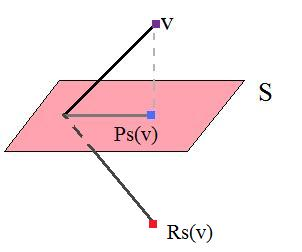
\includegraphics[scale=0.5]{proyeccion}\caption{Proyección y reflexión}
								\end{center}
							\end{figure}
						\end{minipage}
					
				\subsection{Matriz de Householder}
					
					\begin{tikzpicture}
						\node [definicion] (box){%
						\begin{minipage}{0.80\textwidth}
							La matriz de reflexión sobre un subespacio de dimensión $n-1$ que es ortogonal a un vector $\vect{w}$ en un espacio de dimensión $n$ se puede obtener mediante la expresión:
							\begin{align}
								H=I_d-2\frac{\vect{w} \cdot \vect{w}^T}{\vect{w}^T \cdot \vect{w}}
							\end{align}
							Dicha matriz tiene las siguientes propiedades:
							\begin{itemize}
								\item Es involutiva: $H \circ H=I_d$
								\item Es simétrica: $H^T=H$
								\item Es inversible: $\exists H^{-1}$ y $\exists H^{-1}=H$
								\item Es ortogonal: $H^T H=H H^T=I_d$
							\end{itemize}
						\end{minipage}
						};
						\node[fancytitle, right=10pt] at (box.north west) {Propiedades de la proyección};
						\node[fancytitle, rounded corners] at (box.south) {$\aleph$};						
					\end{tikzpicture}
						
				\subsection{Rotaciones en $R^3$}
				
					\begin{tikzpicture}
						\node [definicion] (box){%
						\begin{minipage}{0.80\textwidth}
							Sea $B=\{\vect{v}_1,\vect{v}_2,\vect{v}_3 \}$ una Base Ortonormal (BON) de $R^3$ y sea $T$ la rotación $\theta$ grados alrededor del eje $v_i$:
							\begin{align}
								\text{Rotación sobre } \vect{v}_1 :[T]_B=\begin{bmatrix} {1}&{0}&{0} \\ {0}&{\cos (\theta)}&{-\sin(\theta)} \\ {0}&{\sin (\theta)}&{\cos (\theta)} \end{bmatrix} \\
								\text{Rotación sobre } \vect{v}_2 :[T]_B=\begin{bmatrix} {\cos (\theta)}&{0}&{-\sin(\theta)} \\  {0}&{1}&{0} \\ {\sin (\theta)}&{0}&{\cos (\theta)} \end{bmatrix} \\
								\text{Rotación sobre } \vect{v}_3 :[T]_B=\begin{bmatrix} {\cos (\theta)}&{-\sin(\theta)}&{0} \\ {\sin (\theta)}&{\cos (\theta)}&{0} \\ {0}&{0}&{1} \end{bmatrix} \\
							\end{align}
						\end{minipage}
						};
						\node[fancytitle, right=10pt] at (box.north west) {Rotaciones en $R^3$};
						\node[fancytitle, rounded corners] at (box.south) {$\aleph$};						
					\end{tikzpicture}
						
				\subsection{Proceso de Gram-Schmidt}
				
					\begin{tikzpicture}
						\node [definicion] (box){%
					    \begin{minipage}{0.80\textwidth}
							Dada una base $\{\vect{x}_1,\vect{x}_2,\ldots,\vect{x}_p\}$ para un subespacio $W \in R^n$ defina:
							\begin{enumerate}
								\item $\vect{v}_1=\vect{x}_1$
								\item $\vect{v}_2=\vect{x}_2-\frac{\vect{x}_2 \cdot \vect{v}_1}{\vect{v}_1 \cdot \vect{v}_1}\vect{v}_1$
								\item $\vect{v}_p=\vect{x}_p-\sum_{i=1}^{p-1} \frac{\vect{x}_p \cdot \vect{v}_i}{\vect{v}_i \cdot \vect{v}_i}\vect{v}_i$
							\end{enumerate}
							Entonces $\{ \vect{v}_1,\vect{v}_2,\ldots,\vect{v}_p \}$ es una Base Ortogonal (BOG) de $W$.\\
							
							Si luego se divde a cada componente por la norma de la base se obtiene una Base Ortogonal (BON) de $W$.
					    \end{minipage}
						};
						\node[fancytitle, right=10pt] at (box.north west) {Proceso de Gram-Schmidt};
						\node[fancytitle, rounded corners] at (box.south) {$\aleph$};						
					\end{tikzpicture}
						
				\subsection{Matrices de proyección}
				
					\begin{tikzpicture}
						\node [definicion] (box){%
					    \begin{minipage}{0.80\textwidth}
							Utilizando el producto interno canónico de sobre $K^n$, con $K=R$ o $K=C$.\\
							
							$P \in K^{n \times n}$ es una matriz de proyección si y solo si:
							\begin{align}
								P^2=P \\
								P^H=P
							\end{align}
							Dicha matriz tiene las siguientes propiedades:
							\begin{itemize}
								\item $\col{P}=\nul{P}^\bot$
								\item $P \cdot y=y \Longleftrightarrow y \in \col{P}$
								\item Si $P_S$ es matriz de proyección sobre $S$ y $P_S^\bot$ es matriz de proyección sobre $S^\bot$ entonces $P_S+P_S^\bot=I_d$
								\item Las columnas de $P$ son una base del espacio sobre el cual proyectan
								\item $\rg{P}=\tr{P}$
								\item $\det{P} \neq 0$ si $P\neq I_d$
								\item Si $P_1$ y $P_2$ son matrices de proyección y $P_1 \cdot P_2=P_2 \cdot P_1=0$, entonces $P_1+P_2$ es matriz de proyección y $\rg{P_1+P_2}=\rg{P_1}+\rg{P_2}$
							\end{itemize}		
							Obtención de la matriz de proyección:
							\begin{enumerate}
								\item Sea $Q$ una matriz cuyas columnas son una Base Ortonormal (BON) de $S \subset V$. Entonces la única matriz de proyección sobre $S$ es $[P_S]=Q \cdot Q^T$. La matriz de proyección sobre $S^\bot$ es $[P_S^\bot]=I_d-[P_S]$
								\item Sea $B=\{\vect{v}_1,\ldots,\vect{v}_q \}$ una base de $S$, y $A$ la matriz que tiene por columnas a $\vect{v}_1,\ldots,\vect{v}_q$. Entonces la única matriz de proyección sobre $S$ se obtiene mediante $[P_S]=A\left(A^H A\right)^{-1} A^H=A A^{\#}$	
								\end{enumerate}																			 
					    \end{minipage}
						};
						\node[fancytitle, right=10pt] at (box.north west) {Matriz de proyección};
						\node[fancytitle, rounded corners] at (box.south) {$\aleph$};						
					\end{tikzpicture}
					
				\subsection{Inversas y pseudoinversas}
					
					\begin{tikzpicture}
						\node [definicion] (box){%
					    \begin{minipage}{0.80\textwidth}
							Sea $A \in K^{n \times q} \vert \rg{A}=q$. La matriz pseudoinversa de $A$ es $A^{\#}=\left(A^H A\right)^{-1} A^H$:
							\begin{itemize}
								\item Si $A$ es cuadrada invertible, $A^{-1}=A^{\#}$
								\item $A^{\#} \in R^{q \times n}$
								\item $A^{\#}A=I_{d_{(q)}}$
								\item $A A^{\#}=[P]_{\col{A}}$
								\item $\nul{A A^{\#}}=[\col{A}]^\bot$ 
							\end{itemize}
					    \end{minipage}
						};
						\node[fancytitle, right=10pt] at (box.north west) {Propiedades de la pseudoinversa};
						\node[fancytitle, rounded corners] at (box.south) {$\aleph$};						
					\end{tikzpicture}
					
				\subsection{Cuadrados mínimos}
					
					\begin{tikzpicture}
						\node [definicion] (box){%
					    \begin{minipage}{0.80\textwidth}
							Sea $A \in K^{n \times q}, \vect{x} \in K^q, \vect{b} \in R^n$. Si $Ax=b$ tiene una solución extra, entonces $\vect{b} \in \col{A}$. Si $b \notin \col{A}$, intentamos hallar una solución $\hat{\vect{x}} \in K^q$ (la solución por \textbf{cuadrados mínimos}) tal que:
							\begin{minipage}{0.65\textwidth}
								\begin{itemize}
								\item $\dete{A\hat{\vect{x}}-\vect{b}} < \dete{A\vect{u}-\vect{b}}$, $\forall \vect{u} \in K^q$	
								\item $d(A\hat{\vect{x}},\vect{b}) \leq d(A\vect{u},\vect{b})$, $ \forall \vect{u} \in K^q$
								\item $\dete{A\hat{\vect{x}}} \leq \dete{\vect{b}}$ (Son iguales si $\vect{b} \in \col{A}$)
								\item Ecuaciones normales de cuadrados mínimos: $A^T A \hat{\vect{x}}=A^T \vect{b}=\hat{\vect{b}}$
								\item $A \hat{\vect{x}}=\hat{\vect{b}}=P_{\col{A}}(\vect{b})$ si y solo si:
									\begin{align}
										A\hat{\vect{x}} \in \col{A} \\
										\vect{b}-A\hat{\vect{x}} \in \col{A}^\bot					
									\end{align}									 
								\end{itemize}		
							\end{minipage}
							\begin{minipage}{0.3\textwidth}
								\begin{figure}[H]
									\begin{flushright}
										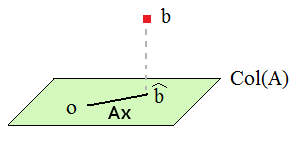
\includegraphics[scale=0.35]{cuad_min}\caption{Cuadrados mínimos}
									\end{flushright}
								\end{figure}
							\end{minipage}
												 
					    \end{minipage}
						};
						\node[fancytitle, right=10pt] at (box.north west) {Cuadrados mínimos};
						\node[fancytitle, rounded corners] at (box.south) {$\aleph$};						
					\end{tikzpicture}
					
					\begin{tikzpicture}
						\node [corolario] (box){%
					    \begin{minipage}{0.80\textwidth}
						 	\begin{enumerate}
						 		\item Si $\hat{\vect{x}}=0$ entonces  $\vect{b} \in [\col{A}]^\bot$. La recíproca solo es cierta si $A$ es invertible.
						 		\item Si las columnas de $A$ son linealmente independientes, la solución por cuadrados mínimos es única y se obtiene mediante:
						 		\begin{align}
						 			\hat{\vect{x}}=(A^T A)^{-1}A^T \vect{b}=A^{\#}\vect{b}
						 		\end{align}
						 		Si las columnas de $A$ son linealmente dependientes, el sistema $A^T A\hat{\vect{x}}=A^T b$ tiene infinitas soluciones, y éstas son de la forma $\hat{\vect{x}}=\hat{\vect{x}}_p+\underbrace{\hat{\vect{x}}_n}_{\in \nul{A}}$
						 		\item Si $\vect{b} \in \col{A}$, entonces toda solución de $A\vect{x}=\vect{b}$ es una solución exacta y por cuadrados mínimos
						 		\item El error de aproximación $\epsilon$ es igual a $\dete{\vect{b}-\hat{\vect{b}}}$
						 	\end{enumerate}
					    \end{minipage}
						};
						\node[fancytitle, right=10pt] at (box.north west) {Propiedades de Cuadrados mínimos};
						\node[fancytitle, rounded corners] at (box.south) {$\aleph$};						
					\end{tikzpicture}
					
					\subsubsection{Norma mínima}
						
						\begin{tikzpicture}
							\node [corolario] (box){%
						    \begin{minipage}{0.80\textwidth}
								La solución por cuadrados mínimos de norma mínima pertenece al espacio $\fil{A}$y se obtiene como:
								\begin{align}
									\tilde{\vect{x}}=A^+ \vect{b}
								\end{align}
								Siendo $A^+$ la \textbf{pseudoinversa de Moore-Penrose} de $A$.
						    \end{minipage}
							};
							\node[fancytitle, right=10pt] at (box.north west) {Pseudoinversa de Moore-Pensore};
							\node[fancytitle, rounded corners] at (box.south) {$\aleph$};						
						\end{tikzpicture}
					
				\subsection{Regresión lineal}				
					
					\begin{tikzpicture}
						\node [definicion] (box){%
					    \begin{minipage}{0.80\textwidth}

					    \end{minipage}
						};
						\node[fancytitle, right=10pt] at (box.north west) {Propiedades de la proyección};
						\node[fancytitle, rounded corners] at (box.south) {$\aleph$};						
					\end{tikzpicture}
					
			\section{Transformaciones lineales}
			\section{Autovalores y Autovectores}
			\section{Matrices hermíticas y simétricas}
			\section{Formas cuadráticas}
			\section{Descomposición en Valores Singulares (DVS)}
			\section{Ecuaciones diferenciales}
			\section{Sistemas de Ecuaciones diferenciales lineales}

\pagebreak
\end{document}
